\subsection{UC17 - Visualizzazione lista prenotazioni (utente base)} \label{usecase:17}
\begin{figure}[H]
  \centering
  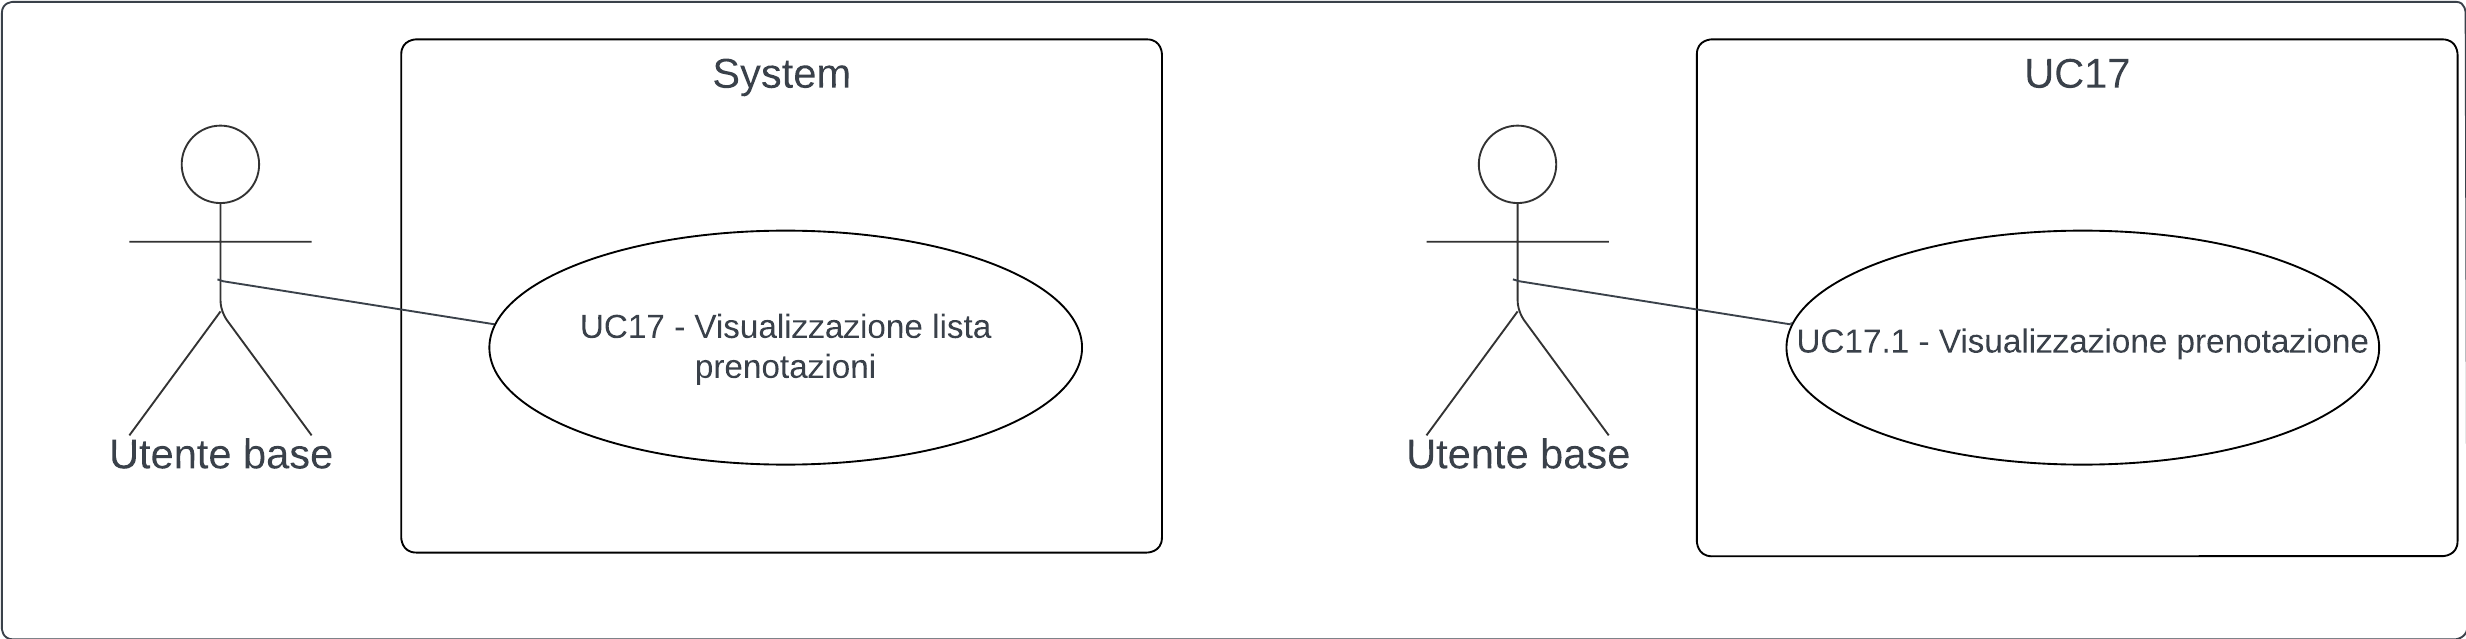
\includegraphics[width=1\textwidth]{ucd/UCD17.png}
  \caption{Visualizzazione lista prenotazioni (utente base)}
\end{figure}
\textbf{Attori}:
\begin{itemize}
    \item Utente base.
\end{itemize}
\textbf{Precondizioni}:
\begin{itemize}
    \item L'utente è connesso al $\textit{sistema}_G$.
\end{itemize}
\textbf{Postcondizioni}:
\begin{itemize}
    \item L'utente visualizza una lista delle prenotazioni con le relative informazioni.
\end{itemize}
\textbf{Scenario principale}:
\begin{enumerate}
    \item L'utente visualizza una lista composta dalle prenotazioni effettuate in precedenza se presenti;
    \item Ogni voce della lista visualizza le informazioni relative alla specifica $\textit{prenotazione}_G$ (\nameref{usecase:17_1}).
\end{enumerate}
\begin{comment}
\textbf{Scenari alternativi}: 
\begin{enumerate}
    \item La lista delle prenotazioni è vuota, viene visualizzato il messaggio: "Non ci sono prenotazioni effettuate"
\end{enumerate}
\end{comment}